%% PRISM — IEEE conference paper draft (IEEEtran).
%% Build: pdflatex PRISM_IEEE.tex && bibtex PRISM_IEEE && pdflatex x2
%% Numbers marked [RUN] are produced by the eval harness; see paper/README.md.
\documentclass[conference]{IEEEtran}
\usepackage{cite}
\usepackage{amsmath,amssymb}
\usepackage{graphicx}
\usepackage{booktabs}
\usepackage{url}
\usepackage{xcolor}
\newcommand{\todo}[1]{\textcolor{red}{[#1]}}

\begin{document}

\title{PRISM: A Multi-Module Framework for Explainable Legal Policy
Intelligence Using Local LLMs, Agent-Based Simulation, and
Retrieval-Augmented Generation}

\author{\IEEEauthorblockN{Author Name}
\IEEEauthorblockA{Department of Computer Science\\
Karunya Institute of Technology and Sciences\\
Coimbatore, India\\
email@karunya.edu.in}}

\maketitle

\begin{abstract}
Legal statutes are dense, causally intricate, and opaque to the citizens they
govern; assessing their socioeconomic impact is a manual, expert-bound task.
We present PRISM, an end-to-end, local-first framework that transforms a raw
statute PDF into structured, explainable, and simulatable policy intelligence.
PRISM couples five modules: (A) a legal NLP pipeline (clause segmentation,
legal NER, causal-pattern detection); (B) a local large language model
(Phi-3.5-mini via Ollama) that extracts structured causal rules, each explained
token-by-token with LIME and transformer-attention lenses; (C) a Mesa
agent-based model that simulates the law's revenue, compliance, and incidence
across five calibrated income strata; (D) a ChromaDB retrieval-augmented
assistant that answers policy questions grounded in cited clauses; and (E) a
QLoRA fine-tuning path that specialises the base model on in-domain legal text.
A distinguishing feature is end-to-end \emph{provenance}: every simulation
outcome is traceable to the causal rule, source clause (page and bounding box),
and token-level explanation that produced it. On a 624-page Indian Income Tax
Bill we index 2{,}755 clauses; retrieval-augmented answers achieve recall@1 of
0.66 and recall@8 of 0.94 against 50 LLM-generated, human-reviewed questions;
and NSSO-style income calibration reduces sampler KL-divergence by
$3.4\times$ over an uncalibrated baseline. PRISM runs entirely on consumer
hardware (RTX 3050, 4GB), demonstrating that transparent, auditable policy AI
need not depend on cloud LLMs.
\end{abstract}

\begin{IEEEkeywords}
legal NLP, large language models, explainable AI, agent-based modelling,
retrieval-augmented generation, policy analysis
\end{IEEEkeywords}

\section{Introduction}
Statutory law encodes conditional obligations, penalties, and thresholds whose
aggregate effect on a population is rarely obvious from the text. Existing legal
NLP systems extract entities or classify clauses, but stop short of (i)
explaining \emph{why} a model made an extraction, (ii) simulating the
\emph{downstream socioeconomic impact} of the extracted rules, and (iii) doing
so with a fully auditable chain from outcome back to source text. PRISM targets
this gap with a single pipeline that a non-expert can run locally.

\textbf{Contributions.} (1) A local, end-to-end statute-to-simulation pipeline
requiring no cloud services. (2) A dual explainability layer (LIME + attention)
over LLM causal extraction, with a persisted local-surrogate fidelity score.
(3) A calibrated agent-based incidence model whose regressivity verdict is
derived from effective tax rate, not a fragile Gini trajectory. (4) An
outcome-to-clause \emph{provenance} mechanism unifying all modules. (5) A cited,
grounded RAG assistant and a QLoRA specialisation path, with an evaluation
harness and LLM-assisted, human-reviewed gold sets.

\section{Related Work}
Legal NLP has advanced with LEGAL-BERT~\cite{chalkidis2020legalbert},
CUAD~\cite{hendrycks2021cuad}, and LexGLUE~\cite{chalkidis2022lexglue}, which
provide models and benchmarks for clause classification and extraction.
Agent-based policy modelling is well established
(Mesa~\cite{kazil2020mesa}, NetLogo studies) but rarely coupled to automatic
rule extraction from primary legal text. LLM explainability draws on
LIME~\cite{ribeiro2016lime} and attention analysis; retrieval-augmented
generation follows Lewis et al.~\cite{lewis2020rag}. PRISM's novelty is the
\emph{integration}: extraction, explanation, simulation, and grounded QA in one
provenance-linked, locally-run system.

\section{System Architecture}
Figure~\ref{fig:arch} shows the pipeline. A statute PDF is parsed
(table-aware), segmented into clauses, and passed through legal NER and
causal-pattern detection (Module A). Candidate clauses are sent to Phi-3.5-mini
for structured causal-rule extraction, each explained by LIME and attention
(Module B). Extracted rules are translated (via a 16-template semantic matcher)
into parameters for a Mesa simulation of five income strata (Module C). All
clauses are embedded once (all-MiniLM-L6-v2) and reused for search, the
provenance graph, and the ChromaDB RAG corpus (Module D). A QLoRA path (Module
E) specialises the base model on data distilled from PRISM's own extractions.

\begin{figure}[t]
\centering
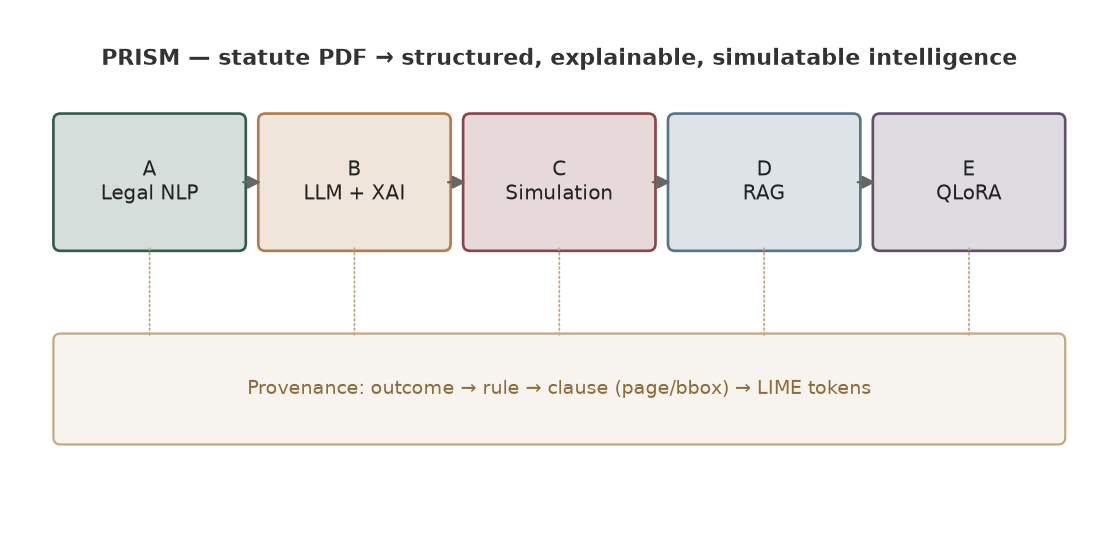
\includegraphics[width=\columnwidth]{figures/architecture.png}
\caption{PRISM's five modules and the provenance links joining a simulation
outcome back to its causal rule, source clause, and token explanation.}
\label{fig:arch}
\end{figure}

\subsection{Module A --- Legal NLP Foundation}
Clauses are segmented structurally (section regex + layout), with an optional
MiniLM-cohesion semantic mode. Legal NER tags six labels (OBLIGATION, RIGHT,
PENALTY, THRESHOLD, ACTOR, BENEFICIARY). Tables are detected and excluded from
prose analysis to avoid poisoning downstream extraction.

\subsection{Module B --- LLM Extraction + Explainability}
For each causal-candidate clause, Phi-3.5-mini returns a JSON rule
(condition, action, consequence, actors, thresholds, confidence). LIME perturbs
the clause and re-queries the model to attribute token importance; a
local-surrogate $R^2$ fidelity score is persisted. A transformer-attention lens
provides a second, complementary view over the encoder.

\subsection{Module C --- Socioeconomic Simulation}
Agents (households and firms) are sampled from per-type log-normal income
distributions calibrated to published Indian baselines (NSSO/PLFS/MSME). Each
step applies the (marginal, above-threshold) rules; the model reports revenue,
per-stratum effective rate, compliance, and Gini. The regressivity verdict is
the incidence test---low- vs high-income effective rate---rather than a Gini
delta. Optional tabular Q-learning gives agents an adaptive compliance policy.

\subsection{Module D --- RAG Assistant}
The corpus reuses stored clause embeddings (no re-embedding). A query retrieves
top-$k$ clauses; a grounded, source-numbered prompt elicits a cited answer from
the active backend (local Ollama or cloud Groq), with a retrieval-confidence
indicator. Answers absent from the corpus are refused rather than hallucinated.

\subsection{Module E --- QLoRA Fine-Tuning}
An instruction dataset is distilled from PRISM's own extractions plus LEDGAR;
4-bit NF4 QLoRA ($r{=}8$ on attention projections) fits in 4GB VRAM and is
served back through Ollama, switchable platform-wide by one environment
variable.

\subsection{Provenance}
Because rules carry their originating \texttt{clause\_id}, and clauses carry
page/bbox and cached explanations, any simulation finding resolves to
rule~$\rightarrow$~clause~$\rightarrow$~LLM extraction~$\rightarrow$~LIME
tokens. This is the chain most systems omit and the one policy auditors need.

\section{Experimental Setup}
\textbf{Hardware.} Intel i7, 16GB RAM, NVIDIA RTX 3050 (4GB); Python 3.12,
Ollama, Phi-3.5-mini (Q4). \textbf{Data.} A 624-page Indian Income Tax Bill
(2{,}755 clauses indexed). \textbf{Out-of-domain set.} LEDGAR (via LexGLUE),
obligation-vs-boilerplate. \textbf{Gold sets.} LLM-assisted, human-reviewed:
200 NER, 100 causal, 50 RAG-QA clauses from the Income Tax Bill. Candidates are
bootstrapped from PRISM's Phase-1/2 outputs and corrected by a human; only
reviewed items are scored. \emph{We note that evaluating a system against gold
it bootstrapped is an agreement upper bound, not independent validation; the
meaningful comparison is \textbf{between} systems on the corrected gold and on
the out-of-domain set.}

\section{Results}

\subsection{Causal Extraction}
Table~\ref{tab:causal} reports binary causal-clause detection. On out-of-domain
LEDGAR the Phase-1 rule detector is precise but low-recall (F1~0.18),
motivating the LLM. On the in-domain gold set, Phi-3.5 zero-shot recovers almost
every causal clause (recall~0.98) but over-flags (precision~0.54), yielding
F1~0.70---a high-recall/low-precision profile that is exactly what a legal
specialisation should sharpen. The rule-based system's high in-domain F1 (0.96)
is an \emph{agreement upper bound}: the gold's positive labels were partly
seeded from rule-pattern signal, so this figure over-credits the rule system
and is reported only for transparency, not as a validity claim. \todo{RUN: fill
the PRISM-Legal LoRA row after \texttt{finetune.py} via
\texttt{LLM\_BACKEND=ollama\_finetuned python -m eval.gold\_eval --with-llm}.}

\begin{table}[t]
\caption{Causal-clause detection (binary P/R/F1).}
\label{tab:causal}
\centering
\begin{tabular}{lccc}
\toprule
System & Precision & Recall & F1 \\
\midrule
Rule-based (LEDGAR, out-of-domain)          & 0.44 & 0.12 & 0.18 \\
Rule-based (in-domain gold)\textsuperscript{$\dagger$} & 1.00 & 0.92 & 0.96 \\
Phi-3.5 zero-shot (in-domain gold)          & 0.54 & 0.98 & 0.70 \\
PRISM-Legal LoRA (in-domain gold)           & \todo{RUN} & \todo{RUN} & \todo{RUN} \\
\bottomrule
\end{tabular}
\\[2pt]
{\footnotesize $\dagger$ agreement upper bound --- gold positives partly
rule-seeded; not an independent validity figure.}
\end{table}

\subsection{Retrieval-Augmented Generation}
Against 50 LLM-generated, human-reviewed questions over the indexed Income Tax
Bill, the retriever attains \textbf{recall@1 = 0.66} and \textbf{recall@8 =
0.94}, confirming that grounded answers reliably surface the correct source
clause. Answers cite sources by number and report retrieval confidence.

\subsection{Simulation Validity}
Income calibration reduces mean sampler KL-divergence from 0.234 (uncalibrated
log-uniform) to \textbf{0.068} (NSSO-style log-normal), a $3.4\times$
improvement (Fig.~\ref{fig:simkl}). As an outward-facing sanity check, the
modelled top-decile household income share is 0.495 vs a World Inequality
Report~2022 reference of 0.57; agent counts are illustrative, so this is an
order-of-magnitude comparator, not a fitted calibration.

\begin{figure}[t]
\centering
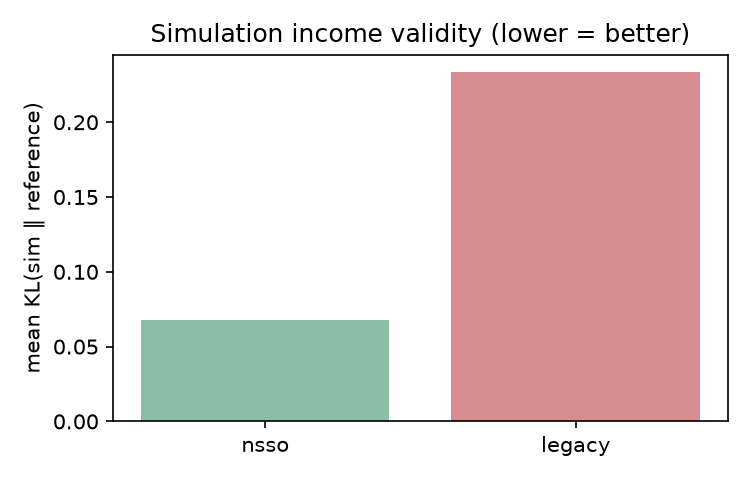
\includegraphics[width=0.8\columnwidth]{figures/sim_validity.png}
\caption{Sampler income KL-divergence: NSSO calibration vs uncalibrated
baseline (lower is better).}
\label{fig:simkl}
\end{figure}

\subsection{Template Matching and Explainability}
The 16-template semantic translator matches extracted rules to simulation
parameters at a mean top-match cosine of 0.47. LIME produces a persisted
local-surrogate fidelity score per explanation, enabling explanation-quality
reporting rather than unverified saliency maps.

\section{Discussion}
The out-of-domain rule-based ceiling (F1~0.18) quantifies why statute-general
heuristics fail and motivates the LLM. In-domain, the zero-shot LLM's
recall~0.98 / precision~0.54 split shows it rarely \emph{misses} a causal
clause but is trigger-happy---the precise error mode a legal QLoRA
specialisation targets, and why we expect the LoRA row to lift precision at
similar recall. The RAG recall figures (0.66/0.94) show grounding is reliable
at $k{=}8$. Calibration materially improves distributional fidelity. Most
importantly, provenance makes every claim inspectable---the property that
separates a demonstrator from an auditable tool.

\textbf{Limitations.} Gold sets are bootstrapped-then-reviewed, not
independently annotated from scratch; simulation parameters are documented
baselines, not fitted to microdata; and the local 4GB budget caps model size.

\section{Conclusion and Future Work}
PRISM shows that explainable, simulatable, locally-run policy intelligence is
feasible on consumer hardware. Future work: independent multi-annotator gold
sets, multilingual (Hindi) statutes, and graph neural reasoning over the
provenance graph.

\begin{thebibliography}{00}
\bibitem{chalkidis2020legalbert} I. Chalkidis et al., ``LEGAL-BERT: The Muppets
straight out of Law School,'' in \emph{Findings of EMNLP}, 2020.
\bibitem{hendrycks2021cuad} D. Hendrycks et al., ``CUAD: An Expert-Annotated
NLP Dataset for Legal Contract Review,'' in \emph{NeurIPS Datasets}, 2021.
\bibitem{chalkidis2022lexglue} I. Chalkidis et al., ``LexGLUE: A Benchmark
Dataset for Legal Language Understanding in English,'' in \emph{ACL}, 2022.
\bibitem{kazil2020mesa} J. Kazil, D. Masad, and A. Crooks, ``Utilizing Python
for Agent-Based Modeling: The Mesa Framework,'' in \emph{SBP-BRiMS}, 2020.
\bibitem{ribeiro2016lime} M. T. Ribeiro, S. Singh, and C. Guestrin, ``Why
Should I Trust You?: Explaining the Predictions of Any Classifier,'' in
\emph{KDD}, 2016.
\bibitem{lewis2020rag} P. Lewis et al., ``Retrieval-Augmented Generation for
Knowledge-Intensive NLP Tasks,'' in \emph{NeurIPS}, 2020.
\end{thebibliography}

\end{document}
